\section{Protein NMR}
NMR (Nuclear Magnetic Resonance) spectroscopy is an experimental technique for 
studying proteins and other biological molecules at atomic resolution.  In 
comparison to other techniques for high-resolution characterization of 
biological molecules, NMR's significance as an experimental technique stems 
from its ability to collect detailed molecular data, from which further 
analysis can derive not only structural information but also dynamics, 
activity, and interactions with other molecules.  The importance of NMR 
spectroscopy to the structural biology community has steadily increased, as 
measured by the number of biologically relevant molecules that have been 
studied using the technique, and the corresponding data deposited into 
publicly available databases -- since 1990, the structures of nearly 9,000 
proteins that were solved using NMR have been deposited in the Protein Data 
Bank (PDB) \cite{pdb}, a facility for the archival and sharing of protein-related 
data, and NMR data is available for over 10,000 proteins in the BioMagnetic 
Resonance Bank (BMRB) \cite{bmrb}, a facility for the archival and sharing of 
specifically NMR-derived data.  The data collected using NMR techniques is 
important to the field of drug design 
\cite{stockman2002drugs, moore2003leveraging, reckel2011proteorhodopsin}, 
as it facilitates identification of potential 
binding partners based on surfaces as well as actual binding partners based on 
chemical shifts, and understanding biological processes.

In order to study proteins in solution using NMR, multi-step processes are 
employed to collect and analyze data.  An example process is shown in 
Figure-\ref{nmr_overview} as a series of independent stages 
\cite{guerry2011automated}.

\begin{figure}
  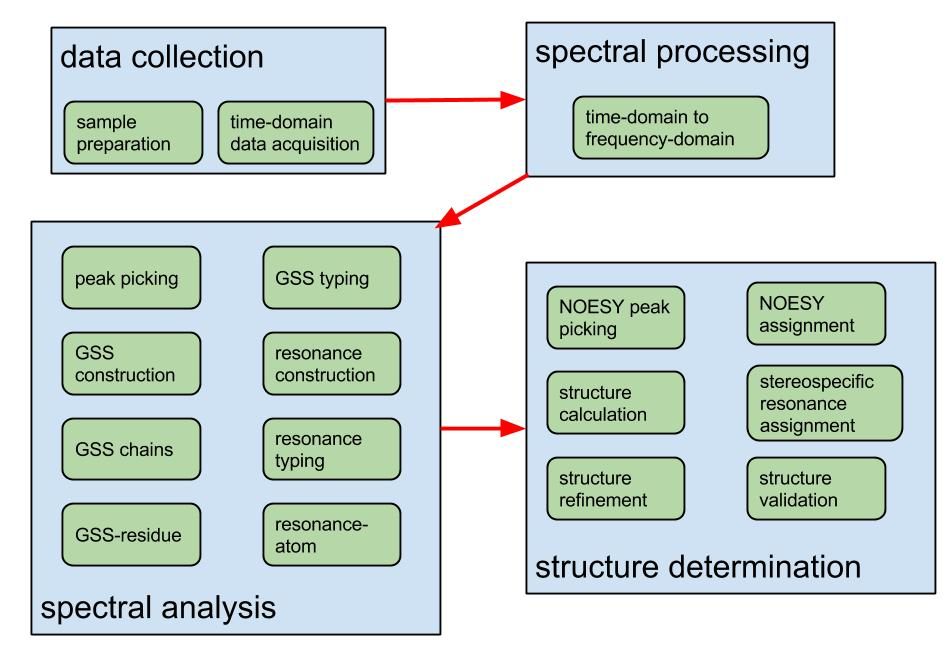
\includegraphics[scale=0.42]{figures/nmr_overview}
  \caption{An overview of the NMR process for protein structure determination}
  \label{nmr_overview}
\end{figure}

First, the protein/molecule of interest is isolated and a concentrated solution 
is obtained.  Then, the solution is placed in an NMR spectrometer and an array 
of time-domain free induction decay (FID)s are collected.  These experiments 
exploit the coupling constants and characteristic chemical shifts of specific 
atoms and functional groups in order to correlate chemical shifts of 
covalently-bound atoms.

Second, spectral processing operates on these FID data sets.  They are 
converted to frequency-domain spectra using tools such as NMRPipe \cite{nmrpipe}
and the Rowland NMR ToolKit \cite{rnmrtk}.  Functions such as 
zero-fills, Fourier transforms, phase shifts, apodizations, and linear 
predictions are applied to the data as a processing pipeline.  These 
functions are used to ensure that the spectra are amenable to further 
analysis, by optimizing peak size and shape and minimizing processing 
artifacts.

Third is the spectral analysis stage, in which the goal is to identify the 
chemical shifts of individual atoms by process known as resonance assignment.
The spectra may be analyzed using a tool such as XEasy \cite{xeasy}, 
Sparky \cite{sparky}, NMRViewJ \cite{nmrviewj}, or CCPN Analysis \cite{ccpn}.  
In each spectrum, peak-picking is performed, and true signal peaks must 
be identified and separated from peaks caused by noise and artifacts.  
Additionally, signal peaks caused by contaminants must be identified.  
Next, GSSs are identified and constructed \cite{ccpn}. 
A GSS is a network of covalently-bonded resonances visible through 
overlapping NMR experiments.  GSSs are composed of resonances; a 
resonance is an NMR-visible signal that corresponds to an atom appearing 
at a specific chemical shift in one or more experiments \cite{ccpn}.  
The connectivity of resonances in a GSS is exploited 
in through-bond experiments.  GSSs then must be assigned 
connectivities to other GSSs through overlap of mutual resonances, 
amino acid types, and finally specific residues of the sample of interest. 
Resonances must also be assigned to specific atoms \cite{ccpn}, 
with the final result being that specific atoms in the sample of interest 
are assigned chemical shift values.  Currently, 100\% assignments are not 
achievable due to several factors such as data quality, ambiguity,
missing resonances, and metal ions \cite{guerry2011automated}.
Between 80\% and 95\% completion may be required \cite{williamson2009automated}
for successful analysis at later stages.

In the fourth and final stage, the chemical shift assignments are used to 
interpret the other class of experimental NMR data, Nuclear Overhauser Effect 
spectroscopy (NOESY) experiments \cite{noe_kaiser}.  
NOESY experiments use through-space 
transfer of magnetization to identify spatially near pairs of Hydrogen nuclei, 
regardless of the number of chemical bonds between them.  NOESY spectra are 
processed and peak-picked, similarly to through-bond spectra, and resonance 
assignments of peaks made.  The resonance assignments of the NOESY data are 
interpreted to obtain distance restraints, which are then used to calculate 
coarse-grained three-dimensional structures.  The structures may then be 
refined and fine-tuned using a computational tool such as Amber \cite{amber}.  
Unambiguous resonance assignment of NOESY data purely on the basis of chemical 
shift assignments may often be impossible or impractical, due to degenerate 
chemical shifts and to non-stereospecific assignments.  While these 
ambiguities can often be resolved through the collection of additional 
NMR data, the expense involved in doing so may often make it more practical 
to attempt to resolve the ambiguities through a structure determination 
program such as CYANA \cite{cyana2004}.

The massive amount of data involved in a structure determination process --
often on the order of gigabytes -- necessitates the use of computational
tools for data management as well as efficiency of analysis.  To address
specific problems in the NMR analysis process, many software implementations 
of useful data processing algorithms have been created, distributed, and 
maintained in recent years.  Additionally, several groups have 
accelerated the process by producing software tools spanning and integrating 
multiple steps to decrease the necessity for time-consuming human intervention
\cite{abacus_assignment}.
This allows automated or semi-automated structure determination for small 
proteins.  Other groups have built integrated pipelines, using one specific 
tool for each step \cite{baran2004automated, sail_flya}, 
and allowing manual intervention at traditionally 
difficult stages.  Many recent methods re-envision structure determination 
as an iterative process, where the results of a later stage may require the 
researcher to re-evaluate or re-perform an earlier stage \cite{cyana2004}; 
this has been applied to interpretation of NOE-derived 
restraints \cite{aria2003}.  Altogether, the structure determination 
process can often take several months \cite{guerry2011automated}.

In general, while computational tools are able to deliver results relatively 
quickly compared to manual analysis, they may not be able to produce more 
accurate results, especially when the input data is low-quality, irregular, or 
otherwise problematic; this can result in false positives and negatives
\cite{williamson2009automated}.  This is a problem at every stage of spectral
analysis.

This has the consequence that NMR structure determination data analysis 
processes cannot be fully automated if high-quality results are required.  
An effective solution to this problem combines the strengths of the automated 
and manual approaches, in a semi-automated fashion:  computational tools are 
used to quickly perform the majority of analyses such as peak-picking and 
GSS construction, and manual analysis is used to clear up the 
relatively small number of cases involving ambiguities and errors caused 
by problematic or unclear data.  Thus, some amount of manual analysis may 
be required at all stages of the data analysis process 
\cite{guntert2009automated, williamson2009automated}.   
Manual analysis follows a general pattern:
\begin{enumerate}
  \item identification: a feature of the data is identified as amenable to 
  interpretation.  For example, the feature may be a false negative (such as 
  a signal peak misclassified as noise by the automated peak-picker), a false 
  positive (such as an artifactual peak misclassified as signal), or an 
  ambiguity (such as overlapped GSSs, causing clustering algorithms to fail).
  \item pattern recognition: the spectroscopist identifies a potential method 
  for interpreting the feature based on his/her domain knowledge of NMR and 
  experience with interpretation of previous data sets.  For example, such 
  methods may take the form of deductive rules:  if <the data matches a 
  certain pattern>, then <it could be interpreted a certain way>.
  \item application of the rule to the data feature.  The chosen rule is 
  applied, and the result of the interpretation is included back into the 
  data set.  The result may now be used to drive further deductions.
  \item repeat -- go to step 1 to identify features for further interpretations
This method is a form of iterative, sequential deduction.  The key components 
are the ordered series of steps, the state of the data before and after each 
step, and the deductive rules used to make interpretations at each step.  In 
addition, it should be noted that the final data set can not be regenerated 
using automated tools alone if there are any manual modifications made to 
tool output.
\end{enumerate}


\section{An Overview of Scientific Methods and Reproducibility}
The term "science" can refer to both the enterprise of knowledge acquisition 
through empirical means, and the body of knowledge acquired through such means 
\cite{drummond2012reproducible}.
The core of science is the notion of reproducibility 
\cite{russell2013reproducibility, nih2014reproducibility} -- that claims can be 
independently tested and verified.  In science, reproducible knowledge can be 
obtained using a set of general techniques collectively known as "the 
scientific method".  These techniques share many characteristics, most notably:
\begin{itemize}
 \item data collection: observation of a natural phenomenon, in which 
 experiments are performed and the results quantified and recorded
 \item analysis, in which the data collected in an experiment is processed to 
 gain information, knowledge, and understanding
 \item experimental design: inventing and codifying a procedure for data 
 collection which tests specific variables of a system, while preventing 
 other variables from confounding the results
 \item hypotheses, which synthesize and organize the information, knowledge, 
 and understanding gained in order to both explain the observed results and 
 predict the outcomes of further experiments
\end{itemize}

Two example orderings of these basic steps are shown in 
Figure-\ref{scientific_method_pipeline}, in which a rigid structure is
imposed as a sequential pipeline, and Figure-\ref{scientific_method}, which 
is a more flexible method because it allows any step to influence any other 
step.  In general, as both examples illustrate, the core of science is a
method of iterative experimental designing, data collection, analysis, and 
hypothesis formulation, which leads to new experiments, data and analysis,  
and so on, resulting in the acquisition of knowledge about the natural world.
\begin{figure}
  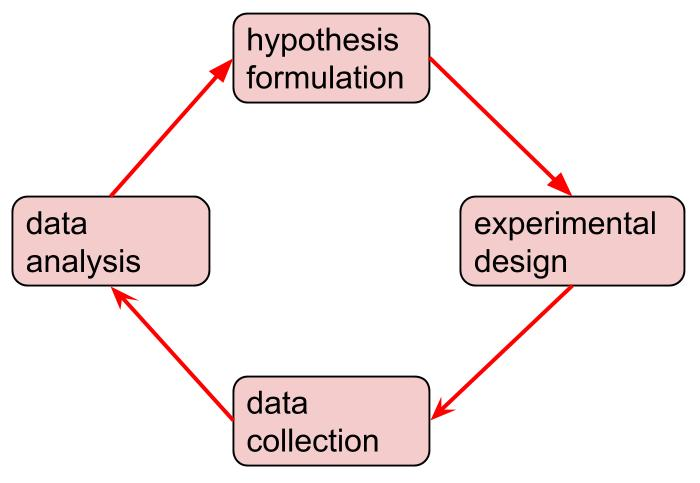
\includegraphics[scale=0.5]{figures/scientific_method_pipeline}
  \caption{A scientific method as a sequential, cyclic pipeline}
  \label{scientific_method_pipeline}
\end{figure}
\begin{figure}
  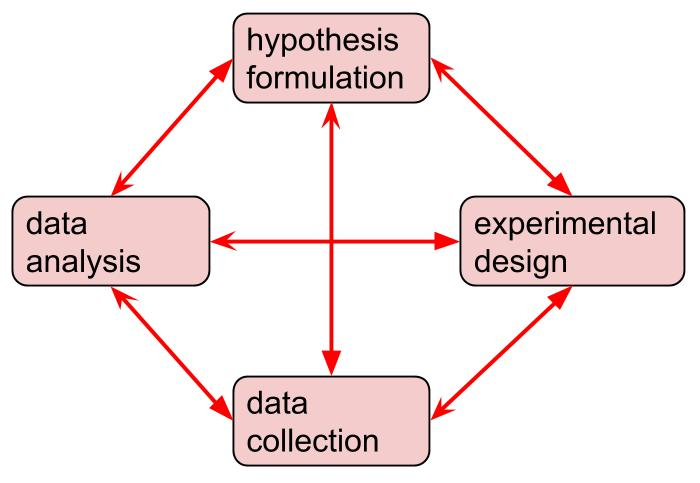
\includegraphics[scale=0.5]{figures/scientific_method}
  \caption{A scientific method in which each step interacts with every other}
  \label{scientific_method}
\end{figure}

A basic principle of scientific methods is that they enable reproducibility.  
In order for scientific results to be reproducible, all components of the 
experimental design, data collection and data analysis steps must be 
reproducible.  These include:
\begin{itemize}

  \item Experimental design.  Our understanding of scientific methods, the 
  significance of reproducibility, and means of achieving reproducibility 
  have evolved along with our experimental methods.  Lab notebooks and journal 
  publications are typical media for enabling reproducibility of experimental 
  designs.  
  The design must be recorded in sufficient detail to convey the key
  points to other scientists.  It may also acknowledge the possibility of 
  confounding variables, and take measures to control for them.
  The appropriate level of detail is neither too much nor too little:
  it should be repeatedly executable such that similar results are obtained 
  -- within expected deviations due to experimental error and variables 
  outside the control of the experiment \cite{drummond2012reproducible}.

  \item Experimental execution.  Lab notebooks and Library Information Systems 
  (LIMS) are also important for recording the details of experiments, including 
  any problems such as contamination.
  When carrying out an experiment, the actual procedure followed should be
  recorded in sufficient detail, including any deviations from the given 
  experimental design and justifications for those changes.
  Biased sampling should also be recognized if possible
  \cite{savovic2012influence, simmons2011false}.

  \item Computational.  As computers continue to play an ever-growing role in 
  science, scientists have noted the problems that indiscriminate computational 
  use poses for reproducibility \cite{donoho2009, peng2011reproducible}.  
  By the early 1990's, researchers began defining reproducible 
  computational analysis \cite{donoho_wavelab}, and describing strategies for 
  achieving it.  A key point is that all tools, scripts, platforms and code 
  available, including the exact versions used
   \cite{ince2012open, nekrutenko2012next, blankenberg2014dissemination}.
  In addition, all parameterizations \cite{landis2012call}, as well
  as input and output data should be recorded.

  \item Analysis.  A further concern of reproducibility is with 
  non-computational analysis; failing to recognize analytical bias and to 
  use appropriate statistical measures has long been a source of 
  irreproducibility in scientific endeavors \cite{sackett1979bias}.
  This has also been previously noted in \cite{ioannidis2005most} 
  in \cite{nuzzo2014statistical, begley2013reproducibility}, 
  and was the focus of a recent Nature special 
  (http://www.nature.com/nature/focus/reproducibility/).
  To ensure reproducibility of analysis, appropriate, necessary, and sufficient
  statistical measures should be used
  \cite{pashler2012replicability, vaux2012numbers}.
  If bias is present in the experimental data, its sources should be recognized
  and accounted for \cite{macarthur2012reproducibility, wagenmakers2012agenda}.
  Additionally, manual changes made during analysis should be recorded.

\end{itemize}

Reproducibility is important to science for several reasons 
\cite{borgman2012conundrum}.  First, it 
provides a means for measuring the quality and usefulness of a study or 
claim.  Second, reproducibility facilitates knowledge transfer between 
peers, which enables fellow researchers to build on the foundation provided 
by a study, whether by extending the experimental design and data collection, 
applying the experiment in a different context, or applying additional analyses 
to existing data.  Third, reproducibility promotes collaboration between fellow 
scientists by enabling sharing of data \cite{rung2013reuse}, 
information, knowledge and experimental 
designs.  Fourth, reproducibility reduces time wastage due to inability to 
replicate results 
\cite{ioannidis2005most, mullard2011reliability, prinz2011reproducibility,
begley2012drug}. 


\section{Reproducible Protein NMR:  Computation and Analysis}
Successful achievement of a reproducible NMR study requires reproducibility at 
each stage of the process.  First, the protocol for expressing, purifying, and 
preparing the sample of interest for experiments inside the NMR spectrometer 
must be reproducible, as well as the exact experimental conditions, 
spectrometer, pulse sequences and collection times used to collect the 
time-domain data must be captured.  Second, the software, platform, functions, 
and parameterizations for spectral processing stage must be captured.  
Third, both the computational results of peak-picking, GSS construction,
GSS assignment, and resonance assignment as well as any manual changes, 
along with the associated deductive process of reasoning, must be captured.  
Fourth, analysis and assignment of NOESY spectra, structure calculation, 
stereospecific resonance assignment and structure refinement must be captured.  
This last stage may also include computational as well as manual analysis 
components.  

This work will focus on reproducibility of the third and fourth stages, 
spectral analysis and structure determination.  Unfortunately, according to 
the definition of reproducible NMR given above, these stages are irreproducible 
because of:
\begin{itemize}
  \item uncaptured primary data: extraneous results, such as GSSs from 
  contaminants, or noise peaks comparable in size to signal peaks
  \item uncaptured primary data: the intermediate results -- tool output before 
  manual analysis, and the state of the data before and after deductions during 
  manual analysis
  \item uncaptured meta data:  the deductive reasoning used during manual analysis
  \item uncaptured primary and meta data: while contemporary NMR databases, 
  such as the BMRB, archive, persist, and disseminate data and analysis 
  results of completed structural, dynamics, and binding studies, the 
  archived data and analysis do not include full information on GSSs 
  and resonances, nor the meta data of manual analysis.  This is because the 
  data is thrown away during the analysis process and not available for deposition.
  \item uncaptured meta data: notes of odd, ambiguous, abnormal, or 
  otherwise unexpected situations noticed during analysis
\end{itemize}

Much work has been done to capture additional data from the assignment process.  
The CCPNMR effort, including the significant projects of CCPN Analysis and the 
CCPN data model \cite{ccpn}, captures includes peaks, atoms, residues, 
resonances, and GSSs, along with other significant NMR data pieces.  
However, there are three shortcomings.  First, intermediate results are not 
captured.  Second, only a subset of these data are deposited into the BMRB.  
This subset typically includes only chemical shift assignments, but not spin 
systems and resonances.   As has already been described, these elements are 
key components of NMR analysis.  Third, the deductive process of reasoning 
is not captured.

Other significant efforts include SPINS \cite{baran2006spins}, 
Sesame \cite{sesame}, and 
the NESG \cite{nesg2005nmr}.  However, much of the previous 
work in this area has focused on project management rather than reproducibility.
SPINS claims to "organize and archive intermediate and final results", but 
only for output files -- it is not designed to capture the key meta data
mentioned above.  Sesame is capable of project management; however, it is 
intended for use in high-throughput studies.  

While the need for integration of automation with occasional manual 
validation and editing has been recognized \cite{baran2006spins}, no 
current systems are capable of combining these features with full 
meta data capturing.  
What is still missing is an approach and tooling for collecting all the primary 
data and meta data of NMR spectral analysis and structure determination.  Much 
time and effort is expended in these stages, but the data is not recorded.  The 
result is that the final data sets deposited into the BMRB are incomplete.

Irreproducible NMR spectral analysis and structure determination causes 
several problems.  As was mentioned in the previous section, the value and 
quality of irreproducible NMR analyses are difficult or impossible to judge; 
irreproducibility limits the ability to transfer knowledge and techniques 
(for interpretation of spectra, resonance assignment, stereospecific resonance 
assignments, etc.) effectively between scientists, as well as preventing close 
collaborations during data analysis and leading to time wastage as 
irreproducible results are discovered and following up on them is found to be 
impossible.  In addition, irreproducibility renders error detection and 
correcting difficult, because the data that would show when, why, and how an 
error occurred would be lost.  It also causes the teaching of analysis methods 
to students and other newcomers to be difficult due to implicit, missing data; 
by capturing and making explicit these data, a more complete picture of the 
process can be discussed and shown.  Finally, irreproducible data may be less 
amenable to future reinterpretation; reinterpreting data is necessary when 
augmenting a data set with additional results, which may fill in missing 
pieces, but may also show the original analysis to be in error.  In short, 
reproducibility of NMR spectral analysis and structure determination will lead 
to better quality results.


\section{An Approach for Reproducible Analysis}
This section outlines one possible approach for rendering analysis reproducible.
As was earlier stated, the key deficiencies causing irreproducibility are 
missing primary data (both extraneous results as well as intermediates), 
missing meta data relating to the deductive process of reasoning employed 
for manual analysis, and undeposited data (both primary and meta).  Therefore, 
the solution will focus on how to capture those data.  In addition, notes for 
identifying potential troublesome and confusing results will be used, as they 
provide a valuable service to future perusers as well as future 
reinterpretation by highlighting mistakes and ambiguities.

\begin{itemize}
  \item Problem: lost primary data:  extraneous results.  Standard approaches use the 
assumption that all peaks are true signal, with no provision for storing peaks 
determined to be processing artifacts or noise.  Such spurious peaks are simply 
deleted and do not show up in the final results.  This is a problem because the 
fact that a peak was found, and later interpreted as noise does not show up in 
the final data set.  The same problem applies to GSSs that are found 
but can not be assigned to any residue of the sample of interest, or are 
believed to correspond to atoms of a contaminant.  Such GSSs should 
be represented in the final data set.

Our approach is to allow any number of peaks and GSSs, and to 
augment them with additional data fields which distinguish between signal, 
noise, contaminants, etc.  This allows one to make a critical distinction 
between: 1) finding/recording a peak based purely on characteristics of 
the spectrum such as volume, height, relative height compared to noise, 
lineshape, and linewidth, and 2) interpreting a peak as signal, noise, 
etc. (and the same for GSSs).  Even peaks and GSSs for 
which no analysis is made can be kept in the data set without encumbering 
assignment of true peaks and GSSs.

  \item Problem: lost primary data: intermediate results.  The output of a 
computational tool, whether used for peak-picking, GSS construction, 
or sequence-specific GSS assignment, is often modified to correct 
mistakes.  This introduces a discrepancy between the output of the tool 
given the input and a suitable parameterization, and the final data set.  
By capturing a snapshot of the output of the tool immediately after it is 
run, and before modifications are made, this discrepancy is rectified.
Similarly, during manual analysis and modification of results, the state of 
the data is continually changing and determines which analyses may be made.  
For example, assignment of a GSS to a residue may allow a further 
unambiguous assignment of a different GSS to a residue (an assignment 
which previously would have been ambiguous) by eliminating one of two 
assignment possibilities based on matching amino acid type.  This shows that 
the state of the data determines what deductions can be made.  Therefore, it 
is important to capture these intermediate states before and after deductions.
The core of the strategy is based on that used by Version Control System (VCS) 
software tools \cite{vcs_concepts, hinsen2009vcs}, which are commonly 
applied for managing source code of 
software projects \cite{loeliger2012git, cvs, svn}.  

These tools were originally implemented in order to manage the change in 
source code over time, while retaining the ability to easily inspect past 
states of the code.  It was found that application of such tools led to 
large increases in productivity, robustness, correctness, and reduced 
faults \cite{fischer2003vcs}.  The core of a VCS is a model for change in data 
over time by storing multiple versions.  Versions are snapshotted, 
descended from previous snapshots, and annotated with a commit message 
which describes the what and the why of the change.  Similarly, in NMR 
during the process of sequential deduction, intermediate states form a 
chain.  By capturing these intermediates, similar advantages are gained 
(as in VCS).  While taking multiple snapshots of a large data set may 
seem wasteful of storage space, it is important to note that there are 
several approaches for compressing the snapshots to eliminate duplication; 
this essentially reduces the wasted space to zero.

  \item Problem: lost meta data: deductive reasons used.  This data describes the 
deductive process of reasoning employed in manually interpreting a feature 
of the primary data.  It is important because it provides the explanation 
of why something was done.

In a VCS, each snapshot is annotated with a commit message that describes 
the how and why of the snapshot -- what problems does it address, what 
features does it add.  Similarly, for capturing the data of the process of 
sequential deduction, the reasoning used describes the change to the data 
set and why it was made.  In order to support the capture of this meta data, 
an extensible library of commonly used deductive reasons enables the user to 
quickly and easily make deductions and describe the reasoning used.  These 
deductive reasons are then referenced in snapshot annotations.

  \item Problem: undeposited data (both primary and meta).  Current depositions to 
the BMRB do not include extraneous results, intermediates, or deductive meta 
data.  

A collaboration with the BMRB will extend the NMR-Star data dictionary to 
support this additional data.  Once the NMR-Star data dictionary supports 
it, spectroscopists will be able to submit complete data sets.

  \item Problem: lost meta data: notes.  As notes indicate the deficiencies and 
potential problems present in a data set, they are valuable to future 
perusers as they highlight how a data set is flawed and how it can be improved.
The CCPN and BMRB data models will be extended to support notes which may 
refer to any aspect of any other piece of primary data in the data set.
\end{itemize}

Additionally, this section will discuss how to effectively put this strategy 
into practice, covering common roadblocks and problems as well as tips and 
suggestions.


\section{Reproducible NMR Data Sets}
In order to prove the utility of the reproducibility approach and annotation 
model in practice, it was applied to a full-scale protein structure 
determination process.  Starting with time-domain data sets of the protein of 
interest, the structure determination process was carried out from start to 
finish, including peak-picking, sequence-specific assignment, NOESY analysis 
and structure calculation.  Intermediate snapshots were captured and 
appropriately annotated.  This data set may now be found deposited in the BMRB.

The data model used was based on the data models of the CCPN project \cite{ccpn}
and of the BMRB \cite{bmrb}, with several 
extensions as previously noted to enable reproducibility.  A library of NMR 
phenomena and their use as deductive inferences rules was constructed.  
These rules were applied for snapshot annotation.

Whereas a single implementation of the previously described strategy is 
here described, in principle the approach is platform-agnostic and 
therefore could be implemented and used by other research group, or added 
into an existing tool as an extension.


\section{Software for Practical Reproducibility}
Software tooling comprises a significant portion of enabling practical 
reproducibility.  High-quality tools can make reproducibility easy, pleasant, 
and safe (in the sense of not error-prone), without placing additional 
unreasonable time, effort, and education demands on potential users.  This 
section will explore a suite of software designed to enable and support 
reproducibility of NMR analysis in various ways.
	
First, a Sparky reproducibility extension has been developed.  This extension
facilitates reproducible data capture during the spectral analysis stage. Sparky 
\cite{sparky} is a popular tool for analysis of NMR data.  One of the major 
strengths of Sparky is its extensibility through user-defined Python modules.  
While its core is written in C++ and is not extensible, a Python module can 
be added without needing to touch the C++ core.  This extension allows
simple data snapshotting, annotation, and capture of extraneous results,
without disrupting the standard Sparky user experience.  The increase in
workload is minimal due to Sparky's keyboard accelerators.

Second, a library for reading and writing of NMR-Star files was implemented.  
NMR-Star is the standard format used by the BMRB for the deposition and 
archival of NMR data.  By storing ongoing data analysis in NMR-Star files, 
users gain the benefits of data integration with the BMRB -- analysis results 
can be uploaded and thereby shared with fellow researchers.  The approach 
taken in implementing and using this parser represents a radical departure 
from standard NMR software techniques; the approach ensures that the 
software will remain easily usable and maintainable as NMR data expands 
and matures.

Third, two tools for working with time- and frequency-domain data sets:  
Connjur Spectrum Translator (ST) and Connjur Workflow Builder (WB).  ST 
translates between various formats of time- and frequency-domain spectra; 
such a tool is necessary because of the input and output requirements of 
many spectral processing tools.  WB provides a high-level interface to 
spectral processing and stores the parameterization, functions, and 
intermediate data sets in a central, relational database.  This means 
that the stage is reproducible.

Fourth, a sample scheduler has been implemented.  This tool facilitates the 
creation of non-uniform sample schedules, which are used to collect time-domain 
data which are non-uniformly sampled in the indirect dimension(s).  Non-uniform 
sampling can help decrease the amount of data collection time required, and 
also help in avoiding the penalties imposed by the necessity of sampling past 
the Rovnyak limit \cite{rovnyak2004accelerated}.  This project included,
a novel data model of sample schedules which included non-uniformity not 
only in the time dimensions but also in the number of transients per FID and 
the quadrature, 
a collection of common algorithms, gathered from descriptions in the 
literature and implemented,
and facilitated easy reproducibility of sample schedule creation by capturing
the parameterization.


\section{CONNJUR is Free and Open Source}
All software developed by the CONNJUR team is released under standard open 
source licenses and is freely available on our website.  The open source 
movement first became popular as a means for users to get control and legal 
rights over software that they had purchased.  This level of ownership is 
important because it enables users to freely and perpetually use, share, 
inspect, fix, maintain, and improve their software.  Such considerations 
become important in view of the rapid changes that scientific fields -- 
including NMR -- undergo: new datatypes, analyses, statistical measures, 
and protocols are developed, requiring updates to old software or entirely 
new software to be written from scratch.  Open source software provides 
additional value in the context of reproducibility: in order to replicate a
study, one must have access to the exact same computational tools that the 
original study used \cite{ince2012open}.  
This involves both physical access -- in the sense of 
being able to get a program loaded onto a computer -- as well as licensing 
issues: does the second group have the rights to use the software in the 
exact same way as in the original study.

Our belief is that open source software can help mitigate these and other 
problems, as well as aid the field in more effectively dealing with its 
nascent software problem, by leading to adoption of a community development 
model and increased sharing, reducing the barriers to future progress in 
the field.  We can only hope that other research groups place as much value 
as we do on open source licenses, and that adoption of open source development 
models will increase.  


\section{Scope and Significance}
Reproducibility is a key enabler of the success of the scientific approach to 
acquiring knowledge.  This work inspects reproducibility in the field of NMR, 
defines the requirements for data analysis that must be met in order to achieve 
reproducibility, and identifies where current practices fall short.  To remedy 
this situation, a strategy for reproducible data analysis is presented.  This 
strategy is made practical by means of a formal model, support from the BMRB 
\cite{bmrb}, and a software implementation.

